\section{Kundengewinnung Marketing}

- Schritt 5: Kundengewinnung Marketing
	- Idee: Mit Hersteller zusammentun
	- Grafik aus Präsentation
	
\begin{figure}[H]
\centering
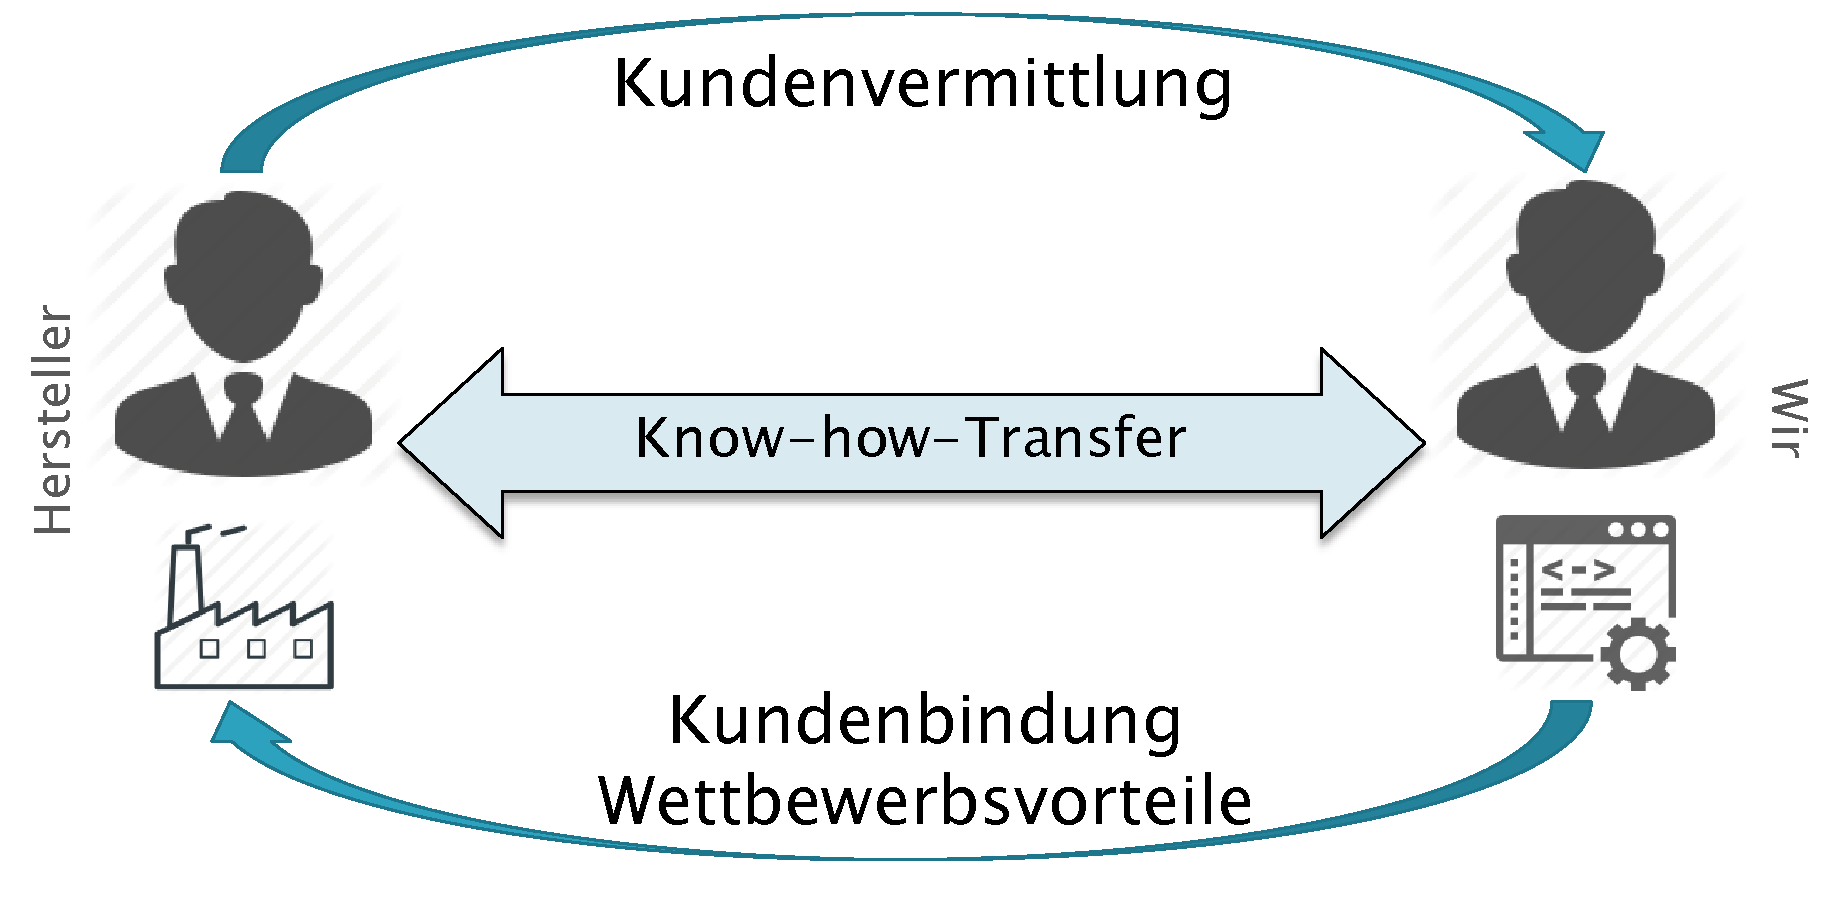
\includegraphics[width=0.7\linewidth]{Bilder/Kundengewinnung}
\caption{Strategie zur Kundengewinnung}
\label{fig:Kundengewinnung}
\end{figure}
	
	
\subsection{Wie gewinnen wir unsere Kunden?}

Um eine erfolgreiche Selbständigkeit aufbauen zu können, müssen wir uns im Vorfeld mit der Frage “Wie gewinnen wir unsere Kunden” auseinandersetzen.
Unsere potentiellen Kunden sind Unternehmen die im produzierenden Gewerbe tätig und von zuverlässigen Atmosphörenöfen abhängig sind. Da wir allerdings keine direkten Kontakte zu diesen Unternehmen haben, möchten wir unsere Dienstleistung nicht für den Endkunden, sondern für einen Hersteller von entsprechenden Öfen anbieten.

Durch unsere langjährige Erfahrung in der Branche sind uns einige namhafte Hersteller bekannt, mit denen eine Kooperation denkbar ist. Um diese zu erreichen, stellen wir uns mit unserer IT-Dienstleistung entsprechend vor. Dabei liefern wir dem Hersteller Antworten auf die Fragen “Warum ist Predective Maintenance wichtig?” und “Warum mit uns?”.

\subsection{Warum ist Predective Maintenance wichtig?}
Mit dem Einsatz von Predictive Maintenance wird die Zuverlässigkeit der Öfen nachhaltig gesteigert. Zusätzlich besteht die Möglichkeit den Endkunden proaktiv und damit rechtzeitig über bevorstehende Probleme zu informieren. Außerdem ist der Hersteller in der Lage seine Serviceleistungen besser zu koordinieren, da Probleme bereits im Vorfeld erkannt werden. Die proaktive Kontaktaufnahme führt zudem zu steigenden Verkaufszahlen im Aftermarket.  Informationen aus den Daten können zusätzlich für Verbesserungen der Öfen genutzt werden.
Insgesamt kann der Hersteller damit sein Image zu einem innovativen und kundenorientierten Anbieter verbessern.

\subsection{Warum mit uns?}
Wir verfügen über das technische Know How und die nötige Erfahrung im Bereich Predective Maintenance und im Bereich des Ofenbaus. Als zuverlässiger Ansprechpartner stehen wir Ihnen auch für komplexe Aufgaben zur Verfügung. Gerne übernehmen wir die Koordination und Konzeption einer für Sie passenden Predictive-Maintenance-Lösung.
	